\documentclass{article}

% content/resources/templates/preamble.tex
\usepackage[margin=0.6in]{geometry}
\author{Milav Dabgar}
\usepackage{amsmath,amssymb,amsthm}
\usepackage{booktabs}
\usepackage{multirow}
\usepackage{xcolor}
\usepackage{tcolorbox}
\tcbuselibrary{breakable,skins}
\usepackage[colorlinks=true,linkcolor=blue]{hyperref}
\usepackage{titlesec}
\usepackage{enumitem}
\usepackage{tikz}
\usepackage{pgfplots}
\usepackage{circuitikz}
\usepackage[version=4]{mhchem}
\usepackage{longtable}
\usepackage{array}
\usepackage{float}
\usepackage{caption}
\usepackage{listings}

\lstset{
  basicstyle=\small\ttfamily,
  breaklines=true,
  breakatwhitespace=false,
  postbreak=\mbox{\textcolor{red}{$\hookrightarrow$}\space},
  float=false,
  numbers=left,
  numberstyle=\tiny\color{gray},
  numbersep=10pt,
  xleftmargin=2em,
  keywordstyle=\color{blue},
  commentstyle=\color{green!60!black},
  stringstyle=\color{purple},
  backgroundcolor=\color{gray!5},
  showstringspaces=false,
  tabsize=2,
  captionpos=b,
  keepspaces=true,
  columns=flexible
}

\pgfplotsset{compat=1.18}
\usetikzlibrary{shapes,arrows,positioning,calc,patterns,decorations.pathmorphing,decorations.markings,arrows.meta}

% Color scheme
\definecolor{headcolor}{RGB}{0,102,204}
\definecolor{keycolor}{RGB}{220,20,60}
\definecolor{solutioncolor}{RGB}{34,139,34}
\definecolor{mnemoniccolor}{RGB}{148,0,211}
\definecolor{codecolor}{RGB}{0,0,100}

% Spacing
\setlength{\parskip}{3pt}
\setlist[itemize]{nosep}
\setlist[enumerate]{nosep}

% Title formatting
\titleformat{\section}{\Large\bfseries\color{headcolor}}{\thesection}{1em}{}
\titleformat{\subsection}{\large\bfseries\color{headcolor}}{\thesubsection}{1em}{}

% Pandoc tightlist compatibility
\providecommand{\tightlist}{%
  \setlength{\itemsep}{0pt}\setlength{\parskip}{0pt}}

% Pandoc longtable compatibility
\newcounter{none}
\def\thenone{}


% content/resources/templates/english-boxes.tex

% Custom environments
\newtcolorbox{solutionbox}{
 breakable,
 enhanced,
 colback=solutioncolor!5!white,
 colframe=solutioncolor!75!black,
 fonttitle=\bfseries,
 title=Solution
}

\newtcolorbox{solutionboxnobreak}{
 colback=solutioncolor!5!white,
 colframe=solutioncolor!75!black,
 fonttitle=\bfseries,
 title=Solution
}

\newtcolorbox{keyformula}{
 breakable,
 enhanced,
 colback=keycolor!5!white,
 colframe=keycolor!75!black,
 fonttitle=\bfseries,
 title=Key Formula
}

\newtcolorbox{mnemonicboxenv}{
 breakable,
 enhanced,
 colback=mnemoniccolor!5!white,
 colframe=mnemoniccolor!75!black,
 fonttitle=\bfseries,
 title=Mnemonic
}

\newcommand{\mnemonicbox}[1]{%
  \begin{mnemonicboxenv}
    #1
  \end{mnemonicboxenv}
}


% Custom commands for GTU solutions
% This file defines semantic commands for consistent formatting

% Question command with automatic formatting
\newcommand{\question}[2]{%
  \section*{Question #1}%
  \textbf{#2}%
}

% OR question variant
\newcommand{\questionor}[2]{%
  \section*{Question #1 OR}%
  \textbf{#2}%
}

% Proper table environment with caption
\newenvironment{answertable}[1]{%
  \begin{table}[htbp]
  \centering
  \caption{#1}
}{%
  \end{table}
}

% Proper figure environment for diagrams
\newenvironment{answerdiagram}[1]{%
  \begin{figure}[htbp]
  \centering
  \caption{#1}
}{%
  \end{figure}
}

% Semantic markup for key terms
\newcommand{\keyword}[1]{\textbf{#1}}
\newcommand{\code}[1]{\texttt{#1}}
\newcommand{\classname}[1]{\texttt{#1}}
\newcommand{\methodname}[1]{\texttt{#1}}

% Proper quotation marks
\newcommand{\mnemonic}[1]{``#1''}

\usetikzlibrary{matrix}

\title{Microprocessor and Microcontroller (4341101) - Summer 2024 Solution}
\date{June 15, 2024}

\begin{document}
\maketitle

\questionmarks{1}{a}{3}
\textbf{Describe any one Port Configuration of 8051 Microcontroller.}

\begin{solutionbox}
\textbf{Answer}:

\begin{center}
\captionof{table}{Port 0 Configuration}
\begin{tabular}{|l|p{10cm}|}
\hline
\textbf{Configuration} & \textbf{Description} \\ \hline
\textbf{Port 0} & Dual-purpose port - 8-bit open drain bidirectional I/O port and multiplexed low address/data bus. External pull-up resistors required for I/O functions. \\ \hline
\end{tabular}
\end{center}

\begin{center}
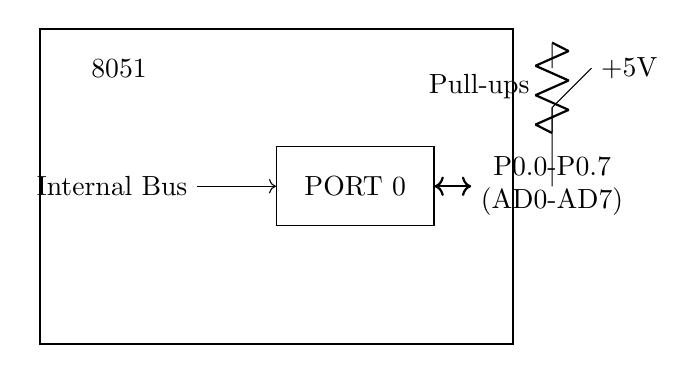
\begin{tikzpicture}[node distance=2.5cm, auto]
    % 8051 Chip Border
    \draw[thick] (0,0) rectangle (6,4);
    \node at (1,3.5) {8051};
    
    % Port 0 Logic Block
    \node[draw, rectangle, minimum width=2cm, minimum height=1cm] (port0) at (4,2) {PORT 0};
    \node[right of=port0, node distance=2.5cm, align=center] (pins) {P0.0-P0.7\\(AD0-AD7)};
    
    % Connection
    \draw[<->, thick] (port0) -- (pins);
    
    % Internal connection
    \draw[<-] (port0.west) -- ++(-1,0) node[anchor=east] {Internal Bus};

    % External Pull-up
    \draw (6.5, 2) -- (6.5, 3) -- (7, 3.5) node[right] {+5V};
    \draw (6.5, 3) to[R, l=Pull-ups] (6.5, 3.5); % Conceptual, simplified
    
    % Note: Better to just use block diagram style for simplicity if circuitikz isn't full
\end{tikzpicture}
\end{center}
\end{solutionbox}
\begin{mnemonicbox}
"PORT 0-PLAD" (Port 0 needs Pull-ups, works as Latch/Address/Data)
\end{mnemonicbox}

\questionmarks{1}{b}{4}
\textbf{Illustrate Microprocessor Architecture.}

\begin{solutionbox}
\textbf{Answer}:

\begin{center}
\captionof{table}{Microprocessor Components}
\begin{tabular}{|l|l|}
\hline
\textbf{Component} & \textbf{Function} \\ \hline
\textbf{ALU} & Performs arithmetic and logical operations \\ \hline
\textbf{Registers} & Temporary storage for data and addresses \\ \hline
\textbf{Control Unit} & Directs operation of processor and data flow \\ \hline
\textbf{Buses} & Pathways for data transfer (address, data, control) \\ \hline
\end{tabular}
\end{center}

\begin{center}
\begin{tikzpicture}[node distance=2cm]
    % CPU Box
    \node [draw, rectangle, minimum width=8cm, minimum height=7cm, fill=black!5, rounded corners] (cpu) {};
    \node [below right] at (cpu.north west) {\textbf{MICROPROCESSOR}};

    % Components
    \node [gtu block, fill=white] (regs) at ([xshift=-2cm, yshift=1.5cm]cpu.center) {REGISTERS\\A, B, C, D\\H, L, SP, PC\\Flags};
    \node [gtu block, fill=white, right of=regs, node distance=4cm] (control) {CONTROL UNIT\\Instruction\\Decoder\\Timing \& Control};
    \node [gtu block, fill=white, below of=regs, node distance=3.5cm] (alu) {ALU};
    
    % Connections
    \draw [gtu arrow, <->] (regs) -- (alu);
    \draw [gtu arrow, <->] (control) -- (regs);
    \draw [gtu arrow] (control) -- (alu);
    
    % Buses
    \node [below of=cpu, node distance=4cm] (buses) {ADDRESS, DATA \& CONTROL BUSES};
    \draw [gtu arrow, <->] (cpu.south) -- (buses);

\end{tikzpicture}
\end{center}
\end{solutionbox}
\begin{mnemonicbox}
"RABC" - "Registers, ALU, Buses, Control"
\end{mnemonicbox}

\questionmarks{1}{c}{7}
\textbf{Compare Von Neumann \& Harvard architecture.}

\begin{solutionbox}
\textbf{Answer}:

\begin{center}
\captionof{table}{Von Neumann vs Harvard Architecture}
\begin{tabular}{|l|p{6cm}|p{6cm}|}
\hline
\textbf{Feature} & \textbf{Von Neumann Architecture} & \textbf{Harvard Architecture} \\ \hline
Memory Buses & Single memory bus for instructions and data & Separate buses for program and data memory \\ \hline
Execution & Sequential execution & Parallel fetch and execute possible \\ \hline
Speed & Slower due to bus bottleneck & Faster due to simultaneous access \\ \hline
Memory Access & Single memory space & Separate memory spaces \\ \hline
Complexity & Simpler design & More complex design \\ \hline
Applications & General-purpose computing & DSP, microcontrollers, embedded systems \\ \hline
Examples & Most PCs, 8085, 8086 & 8051, PIC, ARM Cortex-M \\ \hline
\end{tabular}
\end{center}

\begin{center}
\begin{tikzpicture}[node distance=2cm]
    % Von Neumann
    \node (v_cpu) [gtu block] {CPU};
    \node (v_mem) [gtu block, right of=v_cpu, node distance=3cm] {Memory\\(Code + Data)};
    \draw [gtu arrow, <->] (v_cpu) -- node[above] {Bus} (v_mem);
    \node [below of=v_cpu, node distance=1.5cm] {Von Neumann};

    % Harvard
    \node (h_cpu) [gtu block, right of=v_mem, node distance=4cm] {CPU};
    \node (h_prog) [gtu block, right of=h_cpu, node distance=3cm, yshift=1cm] {Program\\Memory};
    \node (h_data) [gtu block, right of=h_cpu, node distance=3cm, yshift=-1cm] {Data\\Memory};
    \draw [gtu arrow, <->] (h_cpu) -- (h_prog);
    \draw [gtu arrow, <->] (h_cpu) -- (h_data);
    \node [below of=h_cpu, node distance=1.5cm] {Harvard};
\end{tikzpicture}
\end{center}
\end{solutionbox}
\begin{mnemonicbox}
"Harvard Has Separate Streets" (Harvard Has Separate memory paths)
\end{mnemonicbox}

\orquestionmarks{1}{c}{7}
\textbf{Define RISC, CISC, Opcode, Operand, Instruction Cycle, Machine Cycle, and T State.}

\begin{solutionbox}
\textbf{Answer}:

\begin{center}
\captionof{table}{Definitions}
\begin{tabular}{|l|p{10cm}|}
\hline
\textbf{Term} & \textbf{Definition} \\ \hline
\textbf{RISC} & Reduced Instruction Set Computer - architecture with simple instructions optimized for speed \\ \hline
\textbf{CISC} & Complex Instruction Set Computer - architecture with complex, powerful instructions \\ \hline
\textbf{Opcode} & Operation Code - part of instruction that specifies operation to be performed \\ \hline
\textbf{Operand} & Data value or address used in operation \\ \hline
\textbf{Instruction Cycle} & Complete process to fetch, decode and execute an instruction \\ \hline
\textbf{Machine Cycle} & Basic operation like memory read/write (subset of instruction cycle) \\ \hline
\textbf{T-State} & Time state - smallest unit of time in processor operation (clock period) \\ \hline
\end{tabular}
\end{center}

\begin{center}
\begin{tikzpicture}[node distance=2.5cm, auto]
    \node [gtu block] (fetch) {FETCH};
    \node [gtu block, right of=fetch] (decode) {DECODE};
    \node [gtu block, right of=decode] (execute) {EXECUTE};
    
    \draw [gtu arrow] (fetch) -- (decode);
    \draw [gtu arrow] (decode) -- (execute);
    \draw [gtu arrow] (execute) -- ++(0,-1.5) -| (fetch);
    
    \node [below of=decode, node distance=2cm] {\textbf{Instruction Cycle}};
\end{tikzpicture}
\end{center}

\begin{center}
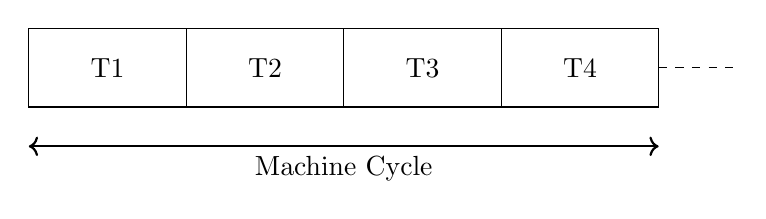
\begin{tikzpicture}
    % T-States
    \foreach \x/\t in {0/T1, 2/T2, 4/T3, 6/T4} {
        \draw (\x,0) rectangle (\x+2,1);
        \node at (\x+1, 0.5) {\t};
    }
    \draw [thick, <->] (0,-0.5) -- (8,-0.5) node[midway, below] {Machine Cycle};
    \draw [dashed] (8,0.5) -- (9,0.5);
\end{tikzpicture}
\end{center}
\end{solutionbox}
\begin{mnemonicbox}
"RICO ITEM" (RISC, CISC, Opcode, Instruction cycle, T-state, Execute, Machine cycle)
\end{mnemonicbox}

\questionmarks{2}{a}{3}
\textbf{Define Data bus, Address bus and Control bus.}

\begin{solutionbox}
\textbf{Answer}:

\begin{center}
\captionof{table}{Bus Definitions}
\begin{tabular}{|l|p{10cm}|}
\hline
\textbf{Bus Type} & \textbf{Definition} \\ \hline
\textbf{Data Bus} & Bidirectional pathway that transfers actual data between microprocessor and peripheral devices \\ \hline
\textbf{Address Bus} & Unidirectional pathway that carries memory/IO device locations to be accessed \\ \hline
\textbf{Control Bus} & Group of signal lines that coordinate and synchronize all system operations \\ \hline
\end{tabular}
\end{center}

\begin{center}
\begin{tikzpicture}[node distance=2.5cm, auto]
    \node [gtu block] (cpu) {CPU};
    
    \draw [->, thick] (cpu.east) -- ++(3,0) node[right, align=left] {Address Bus\\(Memory/IO loc)};
    \draw [<->, thick] (cpu.east) ++(0,-1.5) -- ++(3,0) node[right, align=left] {Data Bus\\(Information)};
    \draw [<->, thick] (cpu.east) ++(0,-3) -- ++(3,0) node[right, align=left] {Control Bus\\(RD, WR, etc.)};
\end{tikzpicture}
\end{center}
\end{solutionbox}
\begin{mnemonicbox}
"ADC" - "Address finds location, Data carries information, Control coordinates operations"
\end{mnemonicbox}

\questionmarks{2}{b}{4}
\textbf{Compare Microprocessor and Microcontroller.}

\begin{solutionbox}
\textbf{Answer}:

\begin{center}
\captionof{table}{Microprocessor vs Microcontroller}
\begin{tabular}{|l|p{6cm}|p{6cm}|}
\hline
\textbf{Feature} & \textbf{Microprocessor} & \textbf{Microcontroller} \\ \hline
Definition & CPU on a single chip & Complete computer system on a chip \\ \hline
Memory & External RAM/ROM needed & Built-in RAM/ROM \\ \hline
I/O Ports & Limited or none on-chip & Multiple I/O ports on-chip \\ \hline
Peripherals & External peripherals needed & Built-in peripherals (timers, ADC, etc.) \\ \hline
Applications & General computing, PCs & Embedded systems, IoT devices \\ \hline
Cost & Higher for complete system & Lower (all-in-one solution) \\ \hline
Power Consumption & Higher & Lower \\ \hline
\end{tabular}
\end{center}
\end{solutionbox}
\begin{mnemonicbox}
"MEMI-CAP" (Memory external/internal, Cost, Applications, Peripherals)
\end{mnemonicbox}

\questionmarks{2}{c}{7}
\textbf{Sketch and explain 8085 block diagram.}

\begin{solutionbox}
\textbf{Answer}:

\begin{center}
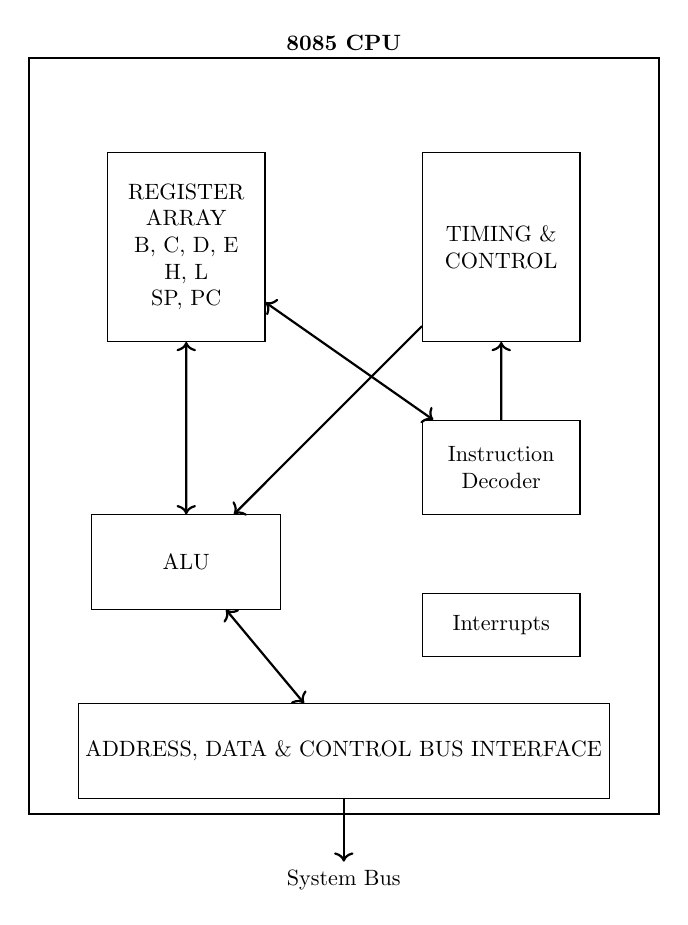
\begin{tikzpicture}[scale=0.8, transform shape]
    % Outer Frame
    \draw[thick] (0,0) rectangle (10,12);
    \node[above] at (5,12) {\textbf{8085 CPU}};

    % Register Array
    \node[draw, rectangle, minimum width=2.5cm, minimum height=3cm, align=center] (regs) at (2.5,9) {REGISTER\\ARRAY\\B, C, D, E\\H, L\\SP, PC};
    
    % Timing & Control
    \node[draw, rectangle, minimum width=2.5cm, minimum height=3cm, align=center] (control) at (7.5,9) {TIMING \&\\CONTROL};
    
    % ALU
    \node[draw, rectangle, minimum width=3cm, minimum height=1.5cm] (alu) at (2.5,4) {ALU};
    
    % Instruction Decoder
    \node[draw, rectangle, minimum width=2.5cm, minimum height=1.5cm, align=center] (decoder) at (7.5,5.5) {Instruction\\Decoder};
    
    % Interrupt Control
    \node[draw, rectangle, minimum width=2.5cm, minimum height=1cm] (interrupt) at (7.5,3) {Interrupts};
    
    % Bus Interface
    \node[draw, rectangle, minimum width=8cm, minimum height=1.5cm, align=center] (bus) at (5,1) {ADDRESS, DATA \& CONTROL BUS INTERFACE};

    % Connections
    \draw[<->, thick] (regs) -- (alu);
    \draw[<->, thick] (decoder) -- (regs);
    \draw[->, thick] (decoder) -- (control);
    \draw[->, thick] (control) -- (alu);
    \draw[<->, thick] (alu) -- (bus);
    
    % External Buses
    \draw[->, thick] (bus.south) -- ++(0,-1) node[below] {System Bus};

\end{tikzpicture}
\end{center}

\textbf{Main Components}:
\begin{itemize}
    \item \textbf{Register Array}: A (Accumulator), Flags, B-L, SP, PC, temp registers
    \item \textbf{ALU}: Performs arithmetic and logical operations
    \item \textbf{Timing \& Control}: Generates control signals, handles interrupts
    \item \textbf{Bus Interface}: Connects CPU to external devices
    \item \textbf{Internal Data Bus}: Links internal components
\end{itemize}
\end{solutionbox}
\begin{mnemonicbox}
"RATBI" - "Registers, ALU, Timing, Buses, Interface"
\end{mnemonicbox}

\orquestionmarks{2}{a}{3}
\textbf{Explain Accumulator, Program Counter and Stack Pointer.}

\begin{solutionbox}
\textbf{Answer}:

\begin{center}
\captionof{table}{Register Functions}
\begin{tabular}{|l|p{10cm}|}
\hline
\textbf{Register} & \textbf{Function} \\ \hline
\textbf{Accumulator (A)} & 8-bit register that stores results of arithmetic and logical operations \\ \hline
\textbf{Program Counter (PC)} & 16-bit register that holds address of next instruction to be executed \\ \hline
\textbf{Stack Pointer (SP)} & 16-bit register that points to current top of stack in memory \\ \hline
\end{tabular}
\end{center}

\begin{center}
\begin{tikzpicture}[node distance=3cm]
    \node [gtu block] (acc) {Accumulator\\(A)};
    \node [gtu block, right of=acc] (pc) {Program Counter\\(PC)};
    \node [gtu block, right of=pc] (sp) {Stack Pointer\\(SP)};
    
    \node [below of=acc, node distance=1.5cm, align=center, font=\small] {Data Ops};
    \node [below of=pc, node distance=1.5cm, align=center, font=\small] {Next Instr Addr};
    \node [below of=sp, node distance=1.5cm, align=center, font=\small] {Stack Top Addr};
\end{tikzpicture}
\end{center}
\end{solutionbox}
\begin{mnemonicbox}
"APS" - "Accumulator Processes, PC Predicts, SP Stacks"
\end{mnemonicbox}

\orquestionmarks{2}{b}{4}
\textbf{Sketch and explain Demultiplexing of Address bus and data bus.}

\begin{solutionbox}
\textbf{Answer}:

\begin{center}
\begin{tikzpicture}[auto, node distance=2.5cm]
    \node [gtu block, minimum width=3cm, minimum height=4cm] (cpu) {8085 CPU};
    \node [gtu block, right of=cpu, node distance=5cm, yshift=-1.5cm] (latch) {74LS373\\Latch};
    
    % Higher Order Address
    \draw [->, thick] (cpu.north east) ++(0,-0.5) -- ++(2,0) node[right] {A15-A8 (Higher Address)};
    
    % Address/Data Bus
    \draw [thick] (cpu.east) ++(0,-1.5) -- ++(1.5,0) coordinate (split);
    \draw [thick] (split) -- (latch.west) node[midway, above] {AD7-AD0};
    \draw [<->, thick] (split) -- ++(0, -1.5) node[below] {Data Bus D7-D0};
    
    % ALE
    \draw [->] (cpu.east) ++(0,-2.5) -- ++(1.5,0) -- (latch.south) node[midway, right] {ALE};
    
    % Latch output
    \draw [->, thick] (latch.east) -- ++(1.5,0) node[right] {A7-A0 (Lower Address)};
    
\end{tikzpicture}
\end{center}

\textbf{Process}:
\begin{enumerate}
    \item \textbf{Multiplexing}: AD0-AD7 pins share address and data signals to reduce pin count
    \item \textbf{Demultiplexing Steps}:
    \begin{itemize}
        \item CPU places address on AD0-AD7 pins
        \item ALE (Address Latch Enable) signal goes HIGH
        \item External latch (74LS373) captures lower address bits
        \item ALE goes LOW, latching the address
        \item AD0-AD7 pins now carry data
    \end{itemize}
\end{enumerate}
\end{solutionbox}
\begin{mnemonicbox}
"ALAD" - "ALE Active, Latch Address, After Data"
\end{mnemonicbox}

\orquestionmarks{2}{c}{7}
\textbf{List any seven features of 8085.}

\begin{solutionbox}
\textbf{Answer}:

\begin{center}
\captionof{table}{8085 Features}
\begin{tabular}{|l|p{10cm}|}
\hline
\textbf{Feature} & \textbf{Description} \\ \hline
\textbf{8-bit Data Bus} & Transfers 8 bits of data in parallel \\ \hline
\textbf{16-bit Address Bus} & Can address up to 64KB of memory ($2^{16}$) \\ \hline
\textbf{Hardware Interrupts} & 5 hardware interrupts (TRAP, RST 7.5, 6.5, 5.5, INTR) \\ \hline
\textbf{Serial I/O} & SID and SOD pins for serial communication \\ \hline
\textbf{Clock Generation} & On-chip clock generator with crystal \\ \hline
\textbf{Instruction Set} & 74 operation codes generating 246 instructions \\ \hline
\textbf{Register Set} & Six 8-bit registers (B,C,D,E,H,L), accumulator, flags, SP, PC \\ \hline
\end{tabular}
\end{center}

\begin{center}
\begin{tikzpicture}[node distance=1.5cm]
    \node [gtu block] (center) {8085 Features};
    
    \node [gtu state, above of=center, node distance=2cm] (bus) {8-bit Data\\16-bit Addr};
    \node [gtu state, right of=center, node distance=3cm] (intr) {5 HW\\Interrupts};
    \node [gtu state, below of=center, node distance=2cm] (serial) {Serial I/O\\SID, SOD};
    \node [gtu state, left of=center, node distance=3cm] (clock) {On-chip\\Clock};
    
    \draw [->] (center) -- (bus);
    \draw [->] (center) -- (intr);
    \draw [->] (center) -- (serial);
    \draw [->] (center) -- (clock);
\end{tikzpicture}
\end{center}
\end{solutionbox}
\begin{mnemonicbox}
"CHAIRS" - "Clock, Hardware interrupts, Address bus, Instruction set, Registers, Serial I/O"
\end{mnemonicbox}

\questionmarks{3}{a}{3}
\textbf{Illustrate any one Timer Mode of 8051.}

\begin{solutionbox}
\textbf{Answer}:

\textbf{Mode 1: 16-bit Timer/Counter}

\begin{center}
\captionof{table}{Timer Mode 1}
\begin{tabular}{|l|l|}
\hline
\textbf{Feature} & \textbf{Description} \\ \hline
\textbf{Timer Structure} & 16-bit timer using THx and TLx registers \\ \hline
\textbf{Operation} & Counts from 0000H to FFFFH, then sets TF flag \\ \hline
\textbf{Counter Size} & Full 16-bit counter ($2^{16} = 65,536$ counts) \\ \hline
\textbf{Registers} & THx (high byte) and TLx (low byte) \\ \hline
\end{tabular}
\end{center}

\begin{center}
\begin{tikzpicture}[auto, node distance=2cm]
    \node [gtu block] (clock) {Clock\\Source};
    \node [gtu block, right of=clock, node distance=3.5cm] (counter) {THx:TLx Counter\\(16-bit)};
    \node [right of=counter, node distance=3cm] (flag) {Overflow Flag\\(TFx)};
    
    \draw [->] (clock) -- node {Gate Control} (counter);
    \draw [->] (counter) -- (flag);
\end{tikzpicture}
\end{center}
\end{solutionbox}
\begin{mnemonicbox}
"MOGC" - "Mode 1 uses Overflow detection, Gate control, Complete 16-bits"
\end{mnemonicbox}

\questionmarks{3}{b}{4}
\textbf{State function of ALE, PSEN, RESET and TXD pin for 8051.}

\begin{solutionbox}
\textbf{Answer}:

\begin{center}
\captionof{table}{Pin Functions}
\begin{tabular}{|l|p{10cm}|}
\hline
\textbf{Pin} & \textbf{Function} \\ \hline
\textbf{ALE} & Address Latch Enable - Provides control signal to latch low byte of address from port 0 \\ \hline
\textbf{PSEN} & Program Store Enable - Read strobe for external program memory access \\ \hline
\textbf{RESET} & Reset input - Forces CPU to initial state when held HIGH for 2 machine cycles \\ \hline
\textbf{TXD} & Transmit Data - Serial port output pin for serial data transmission \\ \hline
\end{tabular}
\end{center}

\begin{center}
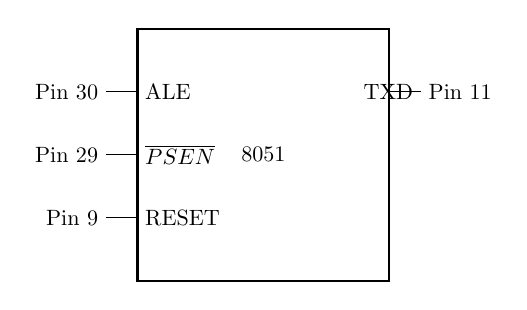
\begin{tikzpicture}[scale=0.8, transform shape]
    \draw[thick] (0,0) rectangle (4,4);
    \node at (2,2) {8051};
    
    \draw (-0.5, 3) -- (0, 3) node[right] {ALE} node[left] at (-0.5, 3) {Pin 30};
    \draw (-0.5, 2) -- (0, 2) node[right] {$\overline{PSEN}$} node[left] at (-0.5, 2) {Pin 29};
    \draw (-0.5, 1) -- (0, 1) node[right] {RESET} node[left] at (-0.5, 1) {Pin 9};
    \draw (4, 3) -- (4.5, 3) node[left] {TXD} node[right] at (4.5, 3) {Pin 11};
\end{tikzpicture}
\end{center}
\end{solutionbox}
\begin{mnemonicbox}
"APTR" - "Address latch, Program store, Total reset, tRansmit data"
\end{mnemonicbox}

\questionmarks{3}{c}{7}
\textbf{Explain functions of each block of 8051 Microcontroller.}

\begin{solutionbox}
\textbf{Answer}:

\begin{center}
\captionof{table}{8051 Components}
\begin{tabular}{|l|p{10cm}|}
\hline
\textbf{Block} & \textbf{Function} \\ \hline
\textbf{CPU} & 8-bit processor that fetches and executes instructions \\ \hline
\textbf{Memory} & 4KB internal ROM and 128 bytes of internal RAM \\ \hline
\textbf{I/O Ports} & Four 8-bit bidirectional I/O ports (P0-P3) \\ \hline
\textbf{Timers/Counters} & Two 16-bit timers/counters for timing and counting \\ \hline
\textbf{Serial Port} & Full-duplex UART for serial communication \\ \hline
\textbf{Interrupts} & Five interrupt sources with two priority levels \\ \hline
\textbf{Clock Circuit} & Provides timing for all operations \\ \hline
\end{tabular}
\end{center}

\begin{center}
\begin{tikzpicture}[node distance=2.5cm]
    % Outer block
    \node [draw, rectangle, minimum width=10cm, minimum height=6cm, fill=black!5, rounded corners] (chip) {};
    \node [below right] at (chip.north west) {\textbf{8051 ARCHITECTURE}};

    % CPU
    \node [gtu block, fill=white] (cpu) at ([xshift=-3cm, yshift=1cm]chip.center) {CPU\\(8-bit)};
    
    % Peripherals
    \node [gtu block, fill=white, right of=cpu, node distance=2.5cm] (mem) {Memory\\RAM/ROM};
    \node [gtu block, fill=white, right of=mem, node distance=2.5cm] (serial) {Serial\\Port};
    \node [gtu block, fill=white, right of=serial, node distance=2.5cm] (io) {I/O Ports\\P0-P3};
    
    \node [gtu block, fill=white, below of=mem, node distance=2.5cm] (timers) {Timers/\\Counters};
    \node [gtu block, fill=white, below of=serial, node distance=2.5cm] (intr) {Interrupts};
    
    % Bus connect
    \draw [gtu arrow, <->] (cpu) -- (mem);
    \draw [gtu arrow, <->] (mem) -- (serial);
    \draw [gtu arrow, <->] (serial) -- (io);
    \draw [gtu arrow, <->] (cpu) |- (timers);
    \draw [gtu arrow, <->] (cpu) |- (intr);
    
    \node [below of=chip, node distance=3.5cm] {Clock Circuit};
\end{tikzpicture}
\end{center}
\end{solutionbox}
\begin{mnemonicbox}
"CRIMSON" - "CPU, RAM/ROM, I/O, Memory, Serial port, Oscillator, iNterrupts"
\end{mnemonicbox}

\orquestionmarks{3}{a}{3}
\textbf{Illustrate any one Serial Communication Mode of 8051.}

\begin{solutionbox}
\textbf{Answer}:

\textbf{Mode 1: 8-bit UART}

\begin{center}
\captionof{table}{Serial Mode 1}
\begin{tabular}{|l|l|}
\hline
\textbf{Feature} & \textbf{Description} \\ \hline
\textbf{Format} & 10 bits (start bit, 8 data bits, stop bit) \\ \hline
\textbf{Baud Rate} & Variable, determined by Timer 1 \\ \hline
\textbf{Data Direction} & Full-duplex (simultaneous transmit and receive) \\ \hline
\textbf{Pins Used} & TXD (P3.1) for transmit, RXD (P3.0) for receive \\ \hline
\end{tabular}
\end{center}

\begin{center}
\begin{tikzpicture}[node distance=2.5cm, auto]
    \node [gtu block] (sbuf) {SBUF};
    \node [gtu block, left of=sbuf, node distance=3.5cm] (timer) {Timer 1\\(Baud Rate)};
    \node [gtu block, right of=sbuf, node distance=3.5cm] (tx) {Transmit\\Shift Reg};
    \node [gtu block, below of=sbuf, node distance=2cm] (rx) {Receive\\Shift Reg};
    
    \draw [->] (timer) -- (sbuf);
    \draw [->] (sbuf) -- (tx);
    \draw [->] (tx) -- node[above] {TXD (P3.1)} ++(2.5,0);
    \draw [<-] (rx) -- node[below] {RXD (P3.0)} ++(2.5,0);
    \draw [->] (rx) -- (sbuf);
\end{tikzpicture}
\end{center}
\end{solutionbox}
\begin{mnemonicbox}
"FADS" - "Format 10-bit, Auto baud from Timer 1, Duplex mode, Standard UART"
\end{mnemonicbox}

\orquestionmarks{3}{b}{4}
\textbf{State function of RXD, INT0, T0 and PROG pin for 8051.}

\begin{solutionbox}
\textbf{Answer}:

\begin{center}
\captionof{table}{Pin Functions}
\begin{tabular}{|l|p{10cm}|}
\hline
\textbf{Pin} & \textbf{Function} \\ \hline
\textbf{RXD (P3.0)} & Receive Data - Serial port input pin for serial data reception \\ \hline
\textbf{INT0 (P3.2)} & External Interrupt 0 - Input that can trigger external interrupt \\ \hline
\textbf{T0 (P3.4)} & Timer 0 - External count input for Timer/Counter 0 \\ \hline
\textbf{PROG (EA)} & Program Enable - When LOW, forces CPU to fetch code from external memory \\ \hline
\end{tabular}
\end{center}

\begin{center}
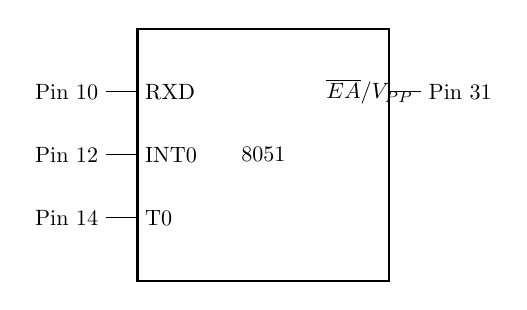
\begin{tikzpicture}[scale=0.8, transform shape]
    \draw[thick] (0,0) rectangle (4,4);
    \node at (2,2) {8051};
    
    \draw (-0.5, 3) -- (0, 3) node[right] {RXD} node[left] at (-0.5, 3) {Pin 10};
    \draw (-0.5, 2) -- (0, 2) node[right] {INT0} node[left] at (-0.5, 2) {Pin 12};
    \draw (-0.5, 1) -- (0, 1) node[right] {T0} node[left] at (-0.5, 1) {Pin 14};
    \draw (4, 3) -- (4.5, 3) node[left] {$\overline{EA}/V_{PP}$} node[right] at (4.5, 3) {Pin 31};
\end{tikzpicture}
\end{center}
\end{solutionbox}
\begin{mnemonicbox}
"RIPE" - "Receive data, Interrupt trigger, Pulse counting, External memory"
\end{mnemonicbox}

\orquestionmarks{3}{c}{7}
\textbf{Describe ALU, PC, DPTR, RS0, RS1, Internal RAM and Internal ROM of 8051.}

\begin{solutionbox}
\textbf{Answer}:

\begin{center}
\captionof{table}{Component Descriptions}
\begin{tabular}{|l|p{10cm}|}
\hline
\textbf{Component} & \textbf{Description} \\ \hline
\textbf{ALU} & Arithmetic Logic Unit - Performs math and logical operations \\ \hline
\textbf{PC} & Program Counter - 16-bit register that points to next instruction \\ \hline
\textbf{DPTR} & Data Pointer - 16-bit register (DPH+DPL) for external memory addressing \\ \hline
\textbf{RS0, RS1} & Register Bank Select bits in PSW - Select one of four register banks \\ \hline
\textbf{Internal RAM} & 128 bytes on-chip RAM (00H-7FH) for variables and stack \\ \hline
\textbf{Internal ROM} & 4KB on-chip ROM (0000H-0FFFH) for program storage \\ \hline
\end{tabular}
\end{center}

\begin{center}
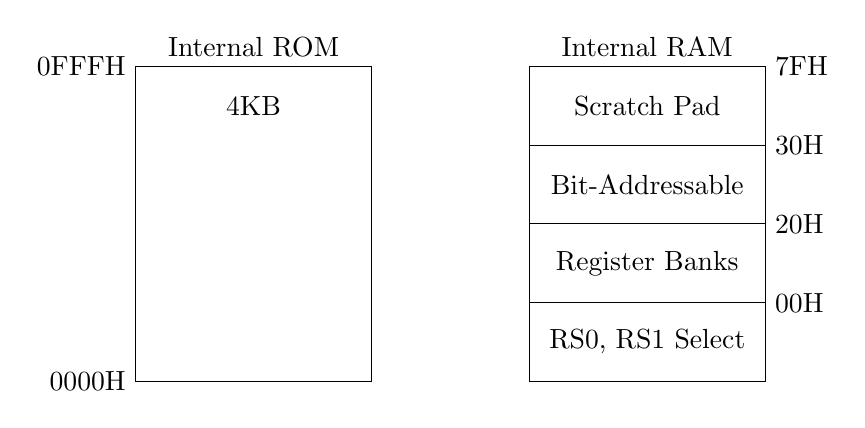
\begin{tikzpicture}
    % ROM
    \node [draw, rectangle, minimum width=3cm, minimum height=4cm, label=above:Internal ROM] (rom) at (0,0) {};
    \node at (0,1.5) {4KB};
    \node [left] at (-1.5, 2) {0FFFH};
    \node [left] at (-1.5, -2) {0000H};
    
    % RAM
    \node [draw, rectangle, minimum width=3cm, minimum height=4cm, label=above:Internal RAM] (ram) at (5,0) {};
    \draw (3.5, 1) -- (6.5, 1);
    \draw (3.5, 0) -- (6.5, 0);
    \draw (3.5, -1) -- (6.5, -1);
    
    \node at (5, 1.5) {Scratch Pad};
    \node at (5, 0.5) {Bit-Addressable};
    \node at (5, -0.5) {Register Banks};
    \node at (5, -1.5) {RS0, RS1 Select};
    
    \node [right] at (6.5, 2) {7FH};
    \node [right] at (6.5, 1) {30H};
    \node [right] at (6.5, 0) {20H};
    \node [right] at (6.5, -1) {00H};
\end{tikzpicture}
\end{center}
\end{solutionbox}
\begin{mnemonicbox}
"APRID" - "ALU Processes, PC Remembers, Register bank select, Internal memory, DPTR points"
\end{mnemonicbox}

\questionmarks{4}{a}{3}
\textbf{Develop an Assembly language program to divide 08H by 02H.}

\begin{solutionbox}
\textbf{Answer}:

\begin{lstlisting}[language={[x86masm]Assembler}]
      MOV A, #08H    ; Load dividend 08H into accumulator
      MOV B, #02H    ; Load divisor 02H into B register
      DIV AB         ; Divide A by B (A=quotient, B=remainder)
      MOV R0, A      ; Store quotient in R0 (04H)
      MOV R1, B      ; Store remainder in R1 (00H)
\end{lstlisting}

\begin{center}
\begin{tikzpicture}[node distance=2cm]
    \node (before) {Before DIV AB};
    \node [gtu block, below of=before, node distance=1cm] (a1) {A = 08H};
    \node [gtu block, below of=a1, node distance=1.5cm] (b1) {B = 02H};
    
    \node [right of=before, node distance=4cm] (after) {After DIV AB};
    \node [gtu block, below of=after, node distance=1cm] (a2) {A = 04H (Quot)};
    \node [gtu block, below of=a2, node distance=1.5cm] (b2) {B = 00H (Rem)};
    
    \draw [->, thick] (a1) -- (a2);
    \draw [->, thick] (b1) -- (b2);
\end{tikzpicture}
\end{center}
\end{solutionbox}
\begin{mnemonicbox}
"LDDS" - "Load dividend, Divisor in B, Divide, Store results"
\end{mnemonicbox}

\questionmarks{4}{b}{4}
\textbf{Develop an Assembly language program to add 76H and 32H.}

\begin{solutionbox}
\textbf{Answer}:

\begin{lstlisting}[language={[x86masm]Assembler}]
      MOV A, #76H    ; Load first number 76H into accumulator
      MOV R0, #32H   ; Load second number 32H into R0
      ADD A, R0      ; Add R0 to A (76H + 32H = A8H)
      MOV R1, A      ; Store result in R1 (A8H)
      JNC DONE       ; Jump if no carry
      MOV R2, #01H   ; If carry occurred, store 1 in R2
DONE: NOP            ; End program
\end{lstlisting}

\begin{center}
\captionof{table}{Calculation}
\begin{tabular}{r c l}
  & 0111 0110 & (76H) \\
+ & 0011 0010 & (32H) \\ \hline
  & 1010 1000 & (A8H) \\
\end{tabular}
\end{center}
\end{solutionbox}
\begin{mnemonicbox}
"LASER" - "Load A, Store second number, Execute addition, Result stored"
\end{mnemonicbox}

\questionmarks{4}{c}{7}
\textbf{What is Addressing mode? Classify it for 8051.}

\begin{solutionbox}
\textbf{Answer}:

\textbf{Addressing Mode}: Method to specify the location of operand/data for an instruction.

\begin{center}
\captionof{table}{8051 Addressing Modes}
\begin{tabular}{|l|l|l|}
\hline
\textbf{Mode} & \textbf{Description} & \textbf{Example} \\ \hline
\textbf{Register} & Operand in register & \code{MOV A, R0} \\ \hline
\textbf{Direct} & Operand at specific memory location & \code{MOV A, 30H} \\ \hline
\textbf{Register Indirect} & Register contains address of operand & \code{MOV A, @R0} \\ \hline
\textbf{Immediate} & Operand is part of instruction & \code{MOV A, \#55H} \\ \hline
\textbf{Indexed} & Base address + offset & \code{MOVC A, @A+DPTR} \\ \hline
\textbf{Bit} & Individual bit addressable & \code{SETB P1.0} \\ \hline
\textbf{Implied} & Operand implied by instruction & \code{RRC A} \\ \hline
\end{tabular}
\end{center}

\begin{center}
\begin{tikzpicture}[node distance=2.5cm, auto]
    % Immediate
    \node [gtu block] (imm) {Immediate\\\#Data};
    \node [gtu block, right of=imm] (dest1) {Dest};
    \draw [->] (imm) -- (dest1);
    
    % Direct
    \node [gtu block, below of=imm, node distance=2cm] (dir) {Address\\(Direct)};
    \node [gtu block, right of=dir] (mem1) {Memory};
    \node [gtu block, right of=mem1] (dest2) {Dest};
    \draw [->] (dir) -- (mem1);
    \draw [->] (mem1) -- (dest2);
    
    % Indirect
    \node [gtu block, below of=dir, node distance=2cm] (ind) {Register\\(@Rp)};
    \node [gtu block, right of=ind] (mem2) {Memory\\Address};
    \node [gtu block, right of=mem2] (dest3) {Dest};
    \draw [->] (ind) -- (mem2);
    \draw [->] (mem2) -- (dest3);
    
\end{tikzpicture}
\end{center}
\end{solutionbox}
\begin{mnemonicbox}
"RIDDIB" - "Register, Immediate, Direct, Data indirect, Indexed, Bit"
\end{mnemonicbox}

\orquestionmarks{4}{a}{3}
\textbf{Develop an Assembly language program to multiply 08H and 02H.}

\begin{solutionbox}
\textbf{Answer}:

\begin{lstlisting}[language={[x86masm]Assembler}]
      MOV A, #08H    ; Load first number 08H into accumulator
      MOV B, #02H    ; Load second number 02H into B register
      MUL AB         ; Multiply A and B (B:A = result)
      MOV R0, A      ; Store low-byte result in R0 (10H)
      MOV R1, B      ; Store high-byte result in R1 (00H)
\end{lstlisting}

\begin{center}
\begin{tikzpicture}[node distance=2cm]
    \node (before) {Before MUL AB};
    \node [gtu block, below of=before, node distance=1cm] (a1) {A = 08H};
    \node [gtu block, below of=a1, node distance=1.5cm] (b1) {B = 02H};
    
    \node [right of=before, node distance=4cm] (after) {After MUL AB};
    \node [gtu block, below of=after, node distance=1cm] (a2) {A = 10H (Low)};
    \node [gtu block, below of=a2, node distance=1.5cm] (b2) {B = 00H (High)};
    
    \draw [->, thick] (a1) -- (a2);
    \draw [->, thick] (b1) -- (b2);
\end{tikzpicture}
\end{center}
\end{solutionbox}
\begin{mnemonicbox}
"LMSR" - "Load numbers, Multiply, Store Result"
\end{mnemonicbox}

\orquestionmarks{4}{b}{4}
\textbf{Develop an Assembly language program to subtract 76H from 32H.}

\begin{solutionbox}
\textbf{Answer}:

\begin{lstlisting}[language={[x86masm]Assembler}]
      MOV A, #32H    ; Load 32H into accumulator
      MOV R0, #76H   ; Load 76H into R0
      CLR C          ; Clear carry flag (borrow flag)
      SUBB A, R0     ; Subtract R0 from A with borrow (32H - 76H = BCH)
      MOV R1, A      ; Store result in R1 (BCH, which represents -44H)
\end{lstlisting}

\begin{center}
\captionof{table}{Calculation}
\begin{tabular}{r c l}
  & 0011 0010 & (32H) \\
- & 0111 0110 & (76H) \\ \hline
  & 1011 1100 & (BCH) \\
\end{tabular}
\end{center}
\end{solutionbox}
\begin{mnemonicbox}
"LESS" - "Load first number, Enable borrow (CLR C), Subtract, Store"
\end{mnemonicbox}

\orquestionmarks{4}{c}{7}
\textbf{List types of instruction set. Explain any three with one example.}

\begin{solutionbox}
\textbf{Answer}:

\begin{center}
\captionof{table}{Instruction Groups}
\begin{tabular}{|l|l|l|}
\hline
\textbf{Group} & \textbf{Description} & \textbf{Example} \\ \hline
\textbf{Arithmetic} & Mathematical operations & \code{ADD A, R0} \\ \hline
\textbf{Logical} & Logical operations & \code{ANL A, \#0FH} \\ \hline
\textbf{Data Transfer} & Move data between locations & \code{MOV A, R7} \\ \hline
\textbf{Branch} & Change program flow & \code{JNZ LOOP} \\ \hline
\textbf{Bit Manipulation} & Operate on individual bits & \code{SETB P1.0} \\ \hline
\textbf{Machine Control} & Control processor operation & \code{NOP} \\ \hline
\end{tabular}
\end{center}

\textbf{Explained Instructions}:
\begin{enumerate}
    \item \textbf{Data Transfer Instructions}: Move data between registers, memory, or I/O ports. Ex: \code{MOV A, 30H} ($A \leftarrow [30H]$).
    \item \textbf{Arithmetic Instructions}: Perform math operations. Ex: \code{ADD A, R0} ($A \leftarrow A + R0$).
    \item \textbf{Logical Instructions}: Perform logical operations. Ex: \code{ANL A, \#0FH} (Masks upper nibble).
\end{enumerate}
\end{solutionbox}
\begin{mnemonicbox}
"BALDM" - "Branch, Arithmetic, Logical, Data transfer, Machine control"
\end{mnemonicbox}

\questionmarks{5}{a}{3}
\textbf{Sketch interfacing of four LEDs with 8051 Microcontroller.}

\begin{solutionbox}
\textbf{Answer}:

\begin{center}
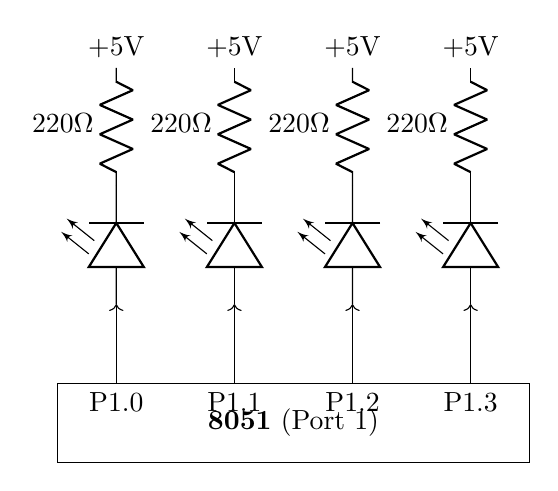
\begin{tikzpicture}[node distance=1.5cm]
    \node [draw, rectangle, minimum width=6cm, minimum height=1cm] (uC) {\textbf{8051} (Port 1)};
    
    % LEDs
    \foreach \i in {0,1,2,3} {
        \draw [->] ([xshift=-2.25cm + \i*1.5cm]uC.north) -- ++(0,1) coordinate (p\i);
        \node [above of=p\i, node distance=0.5cm] (d\i) {}; 
        \draw (p\i) to[leDo] ++(0,1.5) coordinate (r\i);
        \draw (r\i) to[R, l=220$\Omega$] ++(0,1.5) coordinate (v\i);
        \node [above] at (v\i) {+5V};
        \node [below] at ([xshift=-2.25cm + \i*1.5cm]uC.north) {P1.\i};
    }
\end{tikzpicture}
\end{center}
\end{solutionbox}
\begin{mnemonicbox}
"PALS" - "Port pins, Active-low control, LEDs, Simple circuit"
\end{mnemonicbox}

\questionmarks{5}{b}{4}
\textbf{Sketch interfacing of 7 segment LED with 8051 Microcontroller.}

\begin{solutionbox}
\textbf{Answer}:

\begin{center}
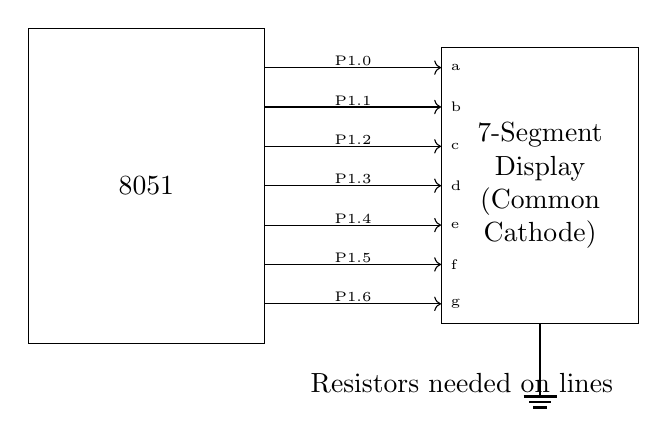
\begin{tikzpicture}[node distance=2cm]
    \node [draw, rectangle, minimum width=3cm, minimum height=4cm] (8051) {8051};
    
    \node [draw, rectangle, minimum width=2.5cm, minimum height=3.5cm, right of=8051, node distance=5cm, align=center] (disp) {7-Segment\\Display\\(Common\\Cathode)};
    
    % Connections
    \foreach \y/\p/\s in {1.5/P1.0/a, 1/P1.1/b, 0.5/P1.2/c, 0/P1.3/d, -0.5/P1.4/e, -1/P1.5/f, -1.5/P1.6/g} {
        \draw [->] (8051.east) ++(0,\y) -- (disp.west |- 0,\y) node[midway, above=-0.1cm, font=\tiny] {\p};
        \node [right, font=\tiny] at (disp.west |- 0,\y) {\s};
    }
    
    % GND
    \draw (disp.south) -- ++(0,-0.5) node[ground] {};
    
    \node at (8051.east) [xshift=2.5cm, yshift=-2.5cm] {Resistors needed on lines};
\end{tikzpicture}
\end{center}

\textbf{Code Example}:
\begin{lstlisting}[language={[x86masm]Assembler}]
; Display digit 5
MOV A, #6DH      ; Segment pattern for 5
MOV P1, A        ; Send to port P1
\end{lstlisting}
\end{solutionbox}
\begin{mnemonicbox}
"SPACE-7" - "Seven Pins, Active segments, Common ground, Easy display"
\end{mnemonicbox}

\questionmarks{5}{c}{7}
\textbf{Explain interfacing of DAC with 8051 Microcontroller and write necessary program.}

\begin{solutionbox}
\textbf{Answer}:

\begin{center}
\begin{tikzpicture}[node distance=2.5cm, auto]
    \node [gtu block, minimum height=3cm] (uC) {8051};
    \node [gtu block, minimum height=3cm, right of=uC, node distance=4cm] (dac) {DAC0808};
    \node [gtu block, right of=dac, node distance=3cm] (opamp) {Op-Amp};
    
    \draw [->, thick] (uC) -- node[above] {P1 (D0-D7)} (dac);
    \draw [->] (dac) -- (opamp);
    \draw [->] (opamp) -- ++(1.5,0) node[right] {Analog Out};
    
    \draw [->] ([yshift=-1cm]uC.east) -- node[below] {P3.0 (CS)} ([yshift=-1cm]dac.west);
    
    \node [below of=dac, node distance=2cm] {Power: $\pm$5V, GND};
\end{tikzpicture}
\end{center}

\textbf{Program for Sawtooth Wave}:
\begin{lstlisting}[language={[x86masm]Assembler}]
START:  MOV R0, #00H     ; Initialize R0 to 0
LOOP:   MOV P1, R0       ; Output value to DAC
        CALL DELAY       ; Wait for some time
        INC R0           ; Increment value
        SJMP LOOP        ; Repeat to create sawtooth wave

DELAY:  MOV R7, #50      ; Load delay counter
DELAY1: MOV R6, #255     ; Inner loop counter
DELAY2: DJNZ R6, DELAY2  ; Decrement R6 until zero
        DJNZ R7, DELAY1  ; Decrement R7 until zero
        RET              ; Return from subroutine
\end{lstlisting}
\end{solutionbox}
\begin{mnemonicbox}
"DICAF" - "Digital input, Increment, Convert to analog, Amplify, Filter"
\end{mnemonicbox}

\orquestionmarks{5}{a}{3}
\textbf{Sketch interfacing of four Switches with 8051 Microcontroller.}

\begin{solutionbox}
\textbf{Answer}:

\begin{center}
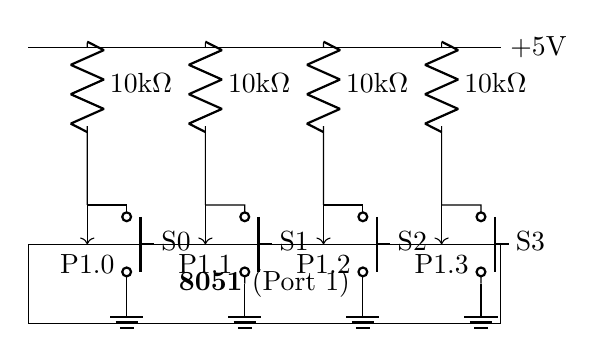
\begin{tikzpicture}[node distance=1.5cm]
    \node [draw, rectangle, minimum width=6cm, minimum height=1cm] (uC) {\textbf{8051} (Port 1)};
    
    % Connection points on uC
    \coordinate (p0) at ([xshift=-2.25cm]uC.north);
    \coordinate (p1) at ([xshift=-0.75cm]uC.north);
    \coordinate (p2) at ([xshift=0.75cm]uC.north);
    \coordinate (p3) at ([xshift=2.25cm]uC.north);

    % Common VCC rail
    \draw (-3, 3) -- (3, 3) node[right] {+5V};

    % Switches and Pull-ups
    \foreach \i/\x in {0/-2.25, 1/-0.75, 2/0.75, 3/2.25} {
        % Pull-up
        \draw (\x, 3) to[R, l=10k$\Omega$] (\x, 2) -- (\x, 1);
        % Connection to Port
        \draw [->] (\x, 1) -- (\x, 0.5); 
        \node [below] at (\x, 0.5) {P1.\i};
        % Switch
        \draw (\x, 1) -- (\x+0.5, 1) to[push button, l=S\i] (\x+0.5, 0) node[ground]{};
    }
\end{tikzpicture}
\end{center}
\end{solutionbox}
\begin{mnemonicbox}
"PIPS" - "Pull-ups, Input pins, Press for zero, Switches"
\end{mnemonicbox}

\orquestionmarks{5}{b}{4}
\textbf{Sketch interfacing of Stepper motor with 8051 Microcontroller.}

\begin{solutionbox}
\textbf{Answer}:

\begin{center}
\begin{tikzpicture}[node distance=2cm, auto]
    \node [gtu block] (uC) {8051};
    \node [gtu block, right of=uC, node distance=3.5cm] (driver) {ULN2003\\Driver};
    \node [gtu block, right of=driver, node distance=3.5cm] (motor) {Stepper\\Motor};
    
    \draw [->, thick] (uC) -- node[above] {P1.0-P1.3} (driver);
    \draw [->, thick] (driver) -- node[above] {Coils A-D} (motor);
    
    \draw [<-] (driver.north) -- ++(0,1) node[above] {+12V};
\end{tikzpicture}
\end{center}

\textbf{Excitation Sequence}:
\begin{center}
\captionof{table}{Step Sequence}
\begin{tabular}{|c|c|c|c|c|c|}
\hline
Step & D (P1.3) & C (P1.2) & B (P1.1) & A (P1.0) & Hex \\ \hline
1 & 0 & 0 & 0 & 1 & 01H \\ \hline
2 & 0 & 0 & 1 & 0 & 02H \\ \hline
3 & 0 & 1 & 0 & 0 & 04H \\ \hline
4 & 1 & 0 & 0 & 0 & 08H \\ \hline
\end{tabular}
\end{center}
\end{solutionbox}
\begin{mnemonicbox}
"CUPS" - "Controller outputs sequence, ULN2003 amplifies, Phases energized, Stepping motion"
\end{mnemonicbox}

\orquestionmarks{5}{c}{7}
\textbf{Explain interfacing of ADC with 8051 Microcontroller and write necessary program.}

\begin{solutionbox}
\textbf{Answer}:

\begin{center}
\begin{tikzpicture}[node distance=2.5cm, auto]
    \node [gtu block, minimum height=3cm] (adc) {ADC0804};
    \node [gtu block, minimum height=3cm, right of=adc, node distance=5cm] (uC) {8051};
    
    \draw [->, thick] (adc) -- node[above] {D0-D7} (uC);
    \node at (2.5, 0.3) {to P1.0-P1.7};
    
    \draw [<-] (adc.west) -- ++(-1.5,0) node[left] {Analog In};
    
    % Control Signals
    \draw [<-] ([yshift=-0.5cm]adc.east) -- node[above] {CS (P3.0)} ([yshift=-0.5cm]uC.west);
    \draw [<-] ([yshift=-1.0cm]adc.east) -- node[above] {RD (P3.1)} ([yshift=-1.0cm]uC.west);
    \draw [<-] ([yshift=-1.5cm]adc.east) -- node[above] {WR (P3.2)} ([yshift=-1.5cm]uC.west);
    \draw [->] ([yshift=-2.0cm]adc.east) -- node[above] {INTR (P3.3)} ([yshift=-2.0cm]uC.west);
    
\end{tikzpicture}
\end{center}

\textbf{Program}:
\begin{lstlisting}[language={[x86masm]Assembler}]
START:  MOV P1, #0FFH    ; Configure P1 as input
READ:   CLR P3.0         ; Enable ADC (CS = 0)
        CLR P3.2         ; Start conversion (WR = 0)
        NOP
        SETB P3.2        ; WR = 1
WAIT:   JB P3.3, WAIT    ; Wait for INTR = 0
        CLR P3.1         ; RD = 0 to read data
        MOV A, P1        ; Read value
        SETB P3.1        ; RD = 1
        SETB P3.0        ; Disable ADC
        MOV R0, A        ; Store result
        SJMP READ        ; Repeat
\end{lstlisting}
\end{solutionbox}
\begin{mnemonicbox}
"CARSW" - "Convert Analog, Read Digital, Start conversion, Wait for completion"
\end{mnemonicbox}

\end{document}
